

\section{The Limit}\label{sec:LimitsWorkingDefn}
The value a function $f$ approaches as its input $x$ approaches some value is said to be the limit of $f$. Limits are essential to the study of calculus and, as we will see, are used in defining continuity, derivatives, and integrals.

Consider the function
$$f(x)=\frac{x^2-1}{x-1}.$$

Notice that $x=1$ does not belong to the domain of $f(x)$.
Regardless, we would like to know how $f(x)$ behaves close to the point $x=1$.
We start with a table of values:
$$\begin{array}{ccc}
\underline{x}&\qquad&\underline{f(x)}\\
0.5&\qquad&1.5\\
0.9&\qquad&1.9\\
0.99&\qquad&1.99\\
1.01&\qquad&2.01\\
1.1&\qquad&2.1\\
1.5&\qquad&2.5\\
\end{array}$$

It appears that for values of $x$ close to $1$ we have that $f(x)$ is close to $2$.
In fact, we can make the values of $f(x)$ as close to $2$ as we like by taking $x$ sufficiently close to $1$.
We express this by saying \ifont{the limit of the function $f(x)$ as $x$ approaches $1$ is equal to $2$} and use the notation:
$$\lim_{x\to 1}f(x)=2.$$
\begin{definition}{Limit (Useable Definition)}{Limit}
In general, we will write
$$\lim_{x\to a}f(x)=L,$$
if we can make the values of $f(x)$ arbitrarily close to $L$ by taking $x$ to be sufficiently close to $a$ (on either side of $a$) but not equal to $a$.
\end{definition}

We read the expression $\lim_{x\to a}f(x)=L$ as ``\ifont{the limit of $f(x)$ as $x$ approaches $a$ is equal to $L$}".
When evaluating a limit, you are essentially answering the following question: 
What number does the function \ifont{approach} while $x$ gets closer and closer to $a$ (but \ifont{not equal} to $a$)?
The phrase \ifont{but not equal to $a$} in the definition of a limit means 
that when finding the limit of $f(x)$ as $x$ approaches $a$ we never actually consider $x=a$.
In fact, as we just saw in the example above, $a$ may not even belong to the domain of $f$.
All that matters for limits is what happens to $f$ close to $a$, not necessarily what happens to $f$ at $a$.







Consider the function $y = \frac{\sin x}{x}$. When $x$ is near the value $ 1 $, what value (if any) is $y$ near?%
 One might think first to look at a graph of this function to approximate the appropriate $y$ values. Consider Figure \ref{fig:zoom_sinx_over_x}, where $y = \frac{\sin x}{x}$ is graphed. For values of $x$ near 1, it seems that $y$ takes on values near $0.85$. In fact, when $x=1$, then $y=\frac{\sin 1}{1} \approx 0.84$, so it makes sense that when $x$ is ``near'' 1, $y$ will be ``near'' $0.84$.





\begin{figure}
	\centering
	\begin{subfigure}[t]{0.5\textwidth}
		\begin{tikzpicture} %[scale=.6]
		\begin{axis}[
		        xmin=0,
		        xmax=1.5,
		        ymin=0,
		        ymax=1,
		       % y=2cm,
		       % x=1cm,
		 %   domain=0.5:1.5,
		    samples=400,
		    axis lines=middle,
		   % xtick = {0.78539, 1.57079, 2.3561,3.1415, 3.92699,4.7123,5.49778,6.28318,7.06858},
		 % xticklabels = {$\frac{\pi}{4}$,$\frac{\pi}{2}$,$\frac{3\pi}{4}$,$\pi $, $\frac{5\pi}{4}$, $\frac{3\pi}{2}$, $\frac{7\pi}{4}$, $2\pi$,},
		 %   ytick={-1,1},
		]
		\addplot [ thick, blue,name path=A, domain = 0.5:1.5] {(sin(deg(x)))/x}; 
		%\draw[red] (axis cs:1.5,4) node {$y=x^2$};
		%\addplot [thick, blue,name path=B,domain=0:2.1] {sqrt(x)};
		%\draw[blue] (axis cs:1.6,.8) node {$y=\sqrt{x}$};
		%\draw[blue] (axis cs: .4,.4) node {\scriptsize $A_1$};
		%\draw[blue] (axis cs:1.6,1.8) node {\scriptsize $A_2$};
		%% \addplot [draw=none,name path=B] {0};     % “fictional” curve
		%  \addplot [\coloronefill] fill between[of = A and B,soft clip={domain=0:2}]; % filling
		\end{axis}
		\end{tikzpicture}
        \label{fig:zoom_sinx_over_x}
        \caption{$\sin(x)/x$ near $x=1$.} 
    \end{subfigure}% 
    \begin{subfigure}[t]{0.5\textwidth}
    \begin{tikzpicture} %[scale=.6]
    \begin{axis}[
            xmin=-1.1,
            xmax=1.1,
            ymin=0,
            ymax=1.5,
           % y=2cm,
           % x=1cm,
       % domain=-1:1,
        samples=400,
        axis lines=middle,
       % xtick = {0.78539, 1.57079, 2.3561,3.1415, 3.92699,4.7123,5.49778,6.28318,7.06858},
     % xticklabels = {$\frac{\pi}{4}$,$\frac{\pi}{2}$,$\frac{3\pi}{4}$,$\pi $, $\frac{5\pi}{4}$, $\frac{3\pi}{2}$, $\frac{7\pi}{4}$, $2\pi$,},
     %   ytick={-1,1},
    ]
    \addplot [ thick, blue,name path=A, domain = -1:-0.01] {(sin(deg(x)))/x}; 
    \addplot [ thick, blue,name path=B, domain = 0.01:1] {(sin(deg(x)))/x}; 
    \draw [fill=white] (axis cs:0,1) circle [radius=1.5pt];
    %\draw[red] (axis cs:1.5,4) node {$y=x^2$};
    %\addplot [thick, blue,name path=B,domain=0:2.1] {sqrt(x)};
    %\draw[blue] (axis cs:1.6,.8) node {$y=\sqrt{x}$};
    %\draw[blue] (axis cs: .4,.4) node {\scriptsize $A_1$};
    %\draw[blue] (axis cs:1.6,1.8) node {\scriptsize $A_2$};
    %% \addplot [draw=none,name path=B] {0};     % “fictional” curve
    %  \addplot [\coloronefill] fill between[of = A and B,soft clip={domain=0:2}]; % filling
    \end{axis}
    \end{tikzpicture}%
        \label{fig:sinx_over_x}
        \caption{$\sin(x)/x$ near $x=0$.}    
    \end{subfigure} 
    \caption{\label{sinx_over_x1}}
\end{figure}





Consider this again at a different value for $x$. When $x$ is near 0, what value (if any) is $y$ near? By considering Figure \ref{sinx_over_x1} \subref{fig:sinx_over_x}, one can see that it seems that $y$ takes on values near $1$. But what happens when $x=0$? We have $$ y \rightarrow \frac{\sin 0}{0} \rightarrow \raisebox{8pt}{\text{``\ }}\frac{0}{0}\raisebox{8pt}{\text{\ ''}}.$$ 
The expression ``$0/0$'' has no value; it is \emph{indeterminate.} \index{limit!indeterminate form}\index{indeterminate form} Such an expression gives no information about what is going on with the function nearby. We cannot find out how $y$ behaves near $x=0$ for this function simply by letting $x=0$. 

\emph{Finding a limit} entails understanding how a function behaves near a particular value of $x$. We approximated $$\lim_{x\to 1} \frac{\sin x}{x} \approx 0.84 \quad \text{ and } \quad \lim_{x\to 0}\frac{\sin x}{x} \approx 1.$$ (We \textit{approximated} these limits, hence used the ``$\approx$'' symbol, since we are working with the pseudo-definition of a limit, not the actual definition.)

Once we have the true definition of a limit, we will find limits \textit{analytically}; that is, exactly using a variety of mathematical tools. For now, we will \textit{approximate} limits both graphically and numerically. Graphing a function can provide a good approximation, though often not very precise. Numerical methods can provide a more accurate approximation. We have already approximated limits graphically, so we now turn our attention to numerical approximations.


Consider again $\lim_{x\to 1}\sin (x)/x$. To approximate this limit numerically, we can create a table of $x$ and $f(x)$ values where $x$ is ``near'' 1. This is done in Table \ref{table:sinx_1}.\par

Notice that for values of $x$ near $1$, we have $\sin (x)/x$ near $0.841$. The $x=1$ row is in bold to highlight the fact that when considering limits, we are \textit{not} concerned with the value of the function at that particular $x$ value; we are only concerned with the values of the function when $x$ is \textit{near} 1. 

\mTable{.3}{Values of $\sin(x)/x$ with $x$ near 1.}{table:sinx_1}{\begin{tabular}{cc}
$x$ & $\sin(x)/x$ \\ \hline 
0.9 & 0.870363 \\
 0.99 & 0.844471 \\
 0.999 & 0.841772 \\
 \textbf{1} & \textbf{0.841471} \\
 1.001 & 0.84117 \\
 1.01 & 0.838447 \\
 1.1 & 0.810189
\end{tabular}
%\caption{Values of $\frac{\sin x}{x}$ for $x$ near 1.}\label{fig:sinx_1_table}}}
%\vskip \baselineskip
}
Now approximate $\lim_{x\to 0} \sin(x)/x$ numerically. We already approximated the value of this limit as 1 graphically in Figure \ref{sinx_over_x1} \subref{fig:sinx_over_x}. Table \ref{table:sinx_2} shows the value of $\sin(x)/x$ for values of $x$ near 0. Ten places after the decimal point are shown to highlight how close to 1 the value of $\sin(x)/x$ gets as $x$ takes on values very near 0. We include the $x=0$ row in bold again to stress that we are not concerned with the value of our function at $x=0$, only on the behaviour of the function \textit{near} 0. 

\mTable{.8}{Values of $\sin(x)/x$ with $x$ near 1.}{table:sinx_2}{\begin{tabular}{cc}
$x$ & $\sin(x)/x$ \\ \hline
 -0.1 & 0.9983341665 \\
 -0.01 & 0.9999833334 \\
 -0.001 & 0.9999998333 \\
 \textbf{0} & \textbf{not defined} \\
 0.001 & 0.9999998333 \\
 0.01 & 0.9999833334 \\
 0.1 & 0.9983341665
 \end{tabular}
% \caption{Values of $\frac{\sin x}{x}$ for $x$ near 0.}\label{fig:sinx_0_table}
}
 
This numerical method gives confidence to say that 1 is a good approximation of $\lim_{x\to 0} \sin(x)/x$; that is, $$\lim_{x\to 0} \sin(x)/x \approx 1.$$ Later we will be able to prove that the limit is \textit{exactly} 1.




We now consider several examples that allow us explore different aspects of the limit concept.\\

 
\begin{example}{Approximating the value of a limit}{exa:ex_limit1}{
Use graphical and numerical methods to approximate $$\lim_{x\to 3} \frac{x^2-x-6}{6x^2-19x+3}.$$}%
\end{example}


\begin{solution}
{To graphically approximate the limit, graph $$y = (x^2-x-6)/(6x^2-19x+3)$$ on a small interval that contains $ 3 $. To numerically approximate the limit, create a table of values where the $x$ values are near $ 3 $. This is done in Figure \ref{fig:limit1} and Table \ref{table:limit1}, respectively.

\mfigure{.5}{ %Graphically approximating a limit in Example \ref{ex_limit1}.
}{fig:limit1}{
\begin{tikzpicture}
\begin{axis}[clip=false, minor x tick num=1,axis y line=middle,axis x line=middle,ymin=.25,ymax=.35,extra y tick labels={},xmin=2.3,xmax=3.7,name=myplot]
\addplot [{\colorone},thick,smooth] coordinates {(2.5,0.321429) (2.61,0.314461) (2.72,0.308094) (2.83,0.302253) (2.94,0.296875) (3.05,0.291908) (3.16,0.287305) (3.27,0.283029) (3.38,0.279046) (3.49,0.275326)};
\end{axis}
\node [right] at (myplot.right of origin) { $x$};
\node [above] at (myplot.above origin) { $y$};
\end{tikzpicture} %
} %
\mTable{.45}{ %Numerically approximating a limit in Example \ref{exa:ex_limit1}.
}{table:limit1}{\begin{tabular}{cc}
$x$ & $\frac{x^2-x-6}{6x^2-19x+3}$ \\ \hline
2.9 & 0.29878 \\
 2.99 & 0.294569 \\
 2.999 & 0.294163 \\
 \textbf{3} & \textbf{not defined}\\
 3.001 & 0.294073 \\
 3.01 & 0.293669 \\
 3.1 & 0.289773
 \end{tabular} %
 }


The graph shows that when $x$ is near 3, the value of $y$ is very near $0.3$. By considering values of $x$ near 3, we see that $y=0.294$ is a better approximation. The graph and the table imply that $$\lim_{x\to 3} \frac{x^2-x-6}{6x^2-19x+3} \approx 0.294.$$ 
}
\end{solution}
 



This example may bring up a few questions about approximating limits (and the nature of limits themselves). 
\begin{enumerate}
\item		If a graph does not produce as good an approximation as a table, why bother with it?
\item		How many values of $x$ in a table are ``enough?'' In the previous example, could we have just used $x=3.001$ and found a fine approximation?
\end{enumerate}

Graphs are useful since they give a visual understanding concerning the behavior of a function. Sometimes a function may act ``erratically'' near certain $x$ values which is hard to discern numerically but very plain graphically. Since graphing utilities are very accessible, it makes sense to make proper use of them.


Since tables and graphs are used only to \textit{approximate} the value of a limit, there is not a firm answer to how many data points are ``enough.'' Include enough so that a trend is clear, and use values (when possible) both less than and greater than the value in question. In Example \ref{ex_limit1}, we used both values less than and greater than 3. Had we used just $x=3.001$, we might have been tempted to conclude that the limit had a value of $0.3$. While this is not far off, we could do better. Using values ``on both sides of 3'' helps us identify trends.\\

\begin{example}{Approximating the value of a limit}{ex_limit2}{
Graphically and numerically approximate the limit of $f(x)$ as $x$ approaches 0, where $$f(x) = \left\{\begin{array}{rl} x+1 & x< 0 \\ -x^2+1 & x > 0 \end{array}\right..$$}
\end{example}


\begin{solution}
{Again we graph $f(x)$ and create a table of its values near $x=0$ to approximate the limit. Note that this is a piecewise defined function, so it behaves differently on either side of 0. Figure \ref{fig:limit2} shows a graph of $f(x)$, and on either side of 0 it seems the $y$ values approach 1. Note that $f(0)$ is not actually defined, as indicated in the graph with the open circle.

\mfigure{.5}{ %Graphically approximating a limit in Example \ref{ex_limit2}.
}{fig:limit2}{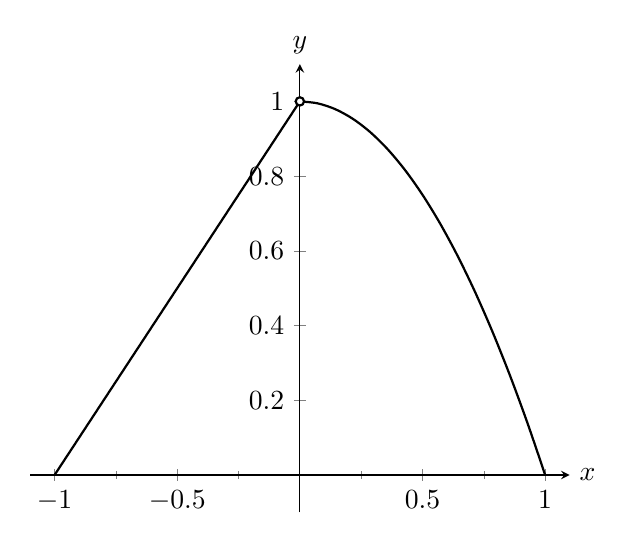
\begin{tikzpicture}
\begin{axis}[minor x tick num=1,axis y line=middle,axis x line=middle,ymin=-.1,ymax=1.1,xmin=-1.1,xmax=1.1,name=myplot]
%%\addplot [{\colorone},thick,smooth] coordinates {(-1.,0.) (-0.89,0.11) (-0.78,0.22) (-0.67,0.33) (-0.56,0.44) (-0.45,0.55) (-0.34,0.66) (-0.23,0.77) (-0.12,0.88) (-0.01,0.99) (0,1) (0.1,0.99) (0.21,0.9559) (0.32,0.8976) (0.43,0.8151) (0.54,0.7084) (0.65,0.5775) (0.76,0.4224) (0.87,0.2431) (1,0) 
%};
\addplot [{\colorone},thick, smooth,domain=-1:0,samples=2] ({x},{x+1});
\addplot [{\colorone},thick, smooth,domain=0:1,samples=15] ({x},{1-x^2});

\filldraw [thick,fill=white] (axis cs:0,1) circle (1.5pt);

\end{axis}
\node [right] at (myplot.right of origin) {  $x$};
\node [above] at (myplot.above origin) {  $y$};
\end{tikzpicture}
%\caption{Graphically approximating $\lim_{x\to 0}f(x)$ in Example \ref{ex_limit2}.}\label{fig:limit2}
}
\mTable{.45}{ %Numerically approximating a limit in Example \ref{ex_limit2}.
}{table:limit2
}{\begin{tabular}{cc}
$x$ & $f(x)$ \\ \hline
-0.1 & 0.9 \\
 -0.01 & 0.99 \\
 -0.001 & 0.999 \\
 0.001 & 0.999999 \\
 0.01 & 0.9999 \\
 0.1 & 0.99
 \end{tabular}}

Table \ref{table:limit2} shows values of $f(x)$ for values of $x$ near 0. It is clear that as $x$ takes on values very near 0, $f(x)$ takes on values very near 1. It turns out that if we let $x=0$ for either ``piece'' of $f(x)$, 1 is returned; this is significant and we'll return to this idea later.

The graph and table allow us to say that $\lim_{x\to 0}f(x) \approx 1$; in fact, we are probably very sure it \textit{equals} 1.
}
\end{solution}




\subsection*{Identifying When Limits Do Not Exist}

A function may not have a limit for all values of $x$. That is, we cannot say $\lim_{x\to c}f(x)=L$ for some numbers $L$ for all values of $c$, for there may not be a number that $f(x)$ is approaching. There are three ways in which a limit may fail to exist. \index{limit!does not exist}
\begin{enumerate}
\item		The function $f(x)$ may approach different values on either side of $c$.
\item		The function may grow without upper or lower bound as $x$ approaches $c$.
\item		The function may oscillate as $x$ approaches $c$.
\end{enumerate}

We'll explore each of these in turn.\\



\begin{example}{Different Values Approached From Left and Right}{ex_no_limit1}{
	Explore why $\ds\lim_{x\to 1} f(x)$ does not exist, where $$f(x) = \left\{\begin{array}{cl} x^2-2x+3 & x\leq 1 \\ x & x>1 \end{array}\right..$$}%	
\end{example}

\begin{solution}
{
A graph of $f(x)$ around $x=1$ and a table are given Figure \ref{fig:nolimit1} and Table \ref{table:nolimit1}, respectively. It is clear that as $x$ approaches $ 1 $, $f(x)$ does not seem to approach a single number. Instead, it seems as though $f(x)$ approaches two different numbers. When considering values of $x$ less than $ 1 $ (approaching $ 1 $ from the left), it seems that $f(x)$ is approaching $ 2 $; when considering values of $x$ greater than $ 1 $ (approaching $ 1 $ from the right), it seems that $f(x)$ is approaching $ 1 $. Recognizing this behavior is important; we'll study this in greater depth later. Right now, it suffices to say that the limit does not exist since $f(x)$ is not approaching one particular value as $x$ approaches $ 1 $.
\mfigure{.5}{Observing no limit as $x\to 1$ in Example \ref{exa:ex_no_limit1}.}{fig:nolimit1}{\begin{tikzpicture}
	\begin{axis}[tick label style={font=\scriptsize},minor x tick num=1,axis y line=middle,axis x line=middle,ymin=-.1,ymax=3.2,xmin=-.1,xmax=2.1,name=myplot]
	
	\addplot [{\colorone},smooth,thick] coordinates {(0.,3.) (0.1,2.81) (0.2,2.64) (0.3,2.49) (0.4,2.36) (0.5,2.25) (0.6,2.16) (0.7,2.09) (0.8,2.04) (0.9,2.01) (1,2)};
	\addplot [{\colorone},smooth,thick] coordinates {(1,1) (1.1,1.1) (1.2,1.2) (1.3,1.3) (1.4,1.4) (1.5,1.5) (1.6,1.6) (1.7,1.7) (1.8,1.8) (1.9,1.9) (2.,2.)
	};
	\filldraw [fill=white,draw={\colorone},thick] (axis cs:1,1) circle (1.5pt);
	\filldraw [fill={\colorone},{\colorone}] (axis cs:1,2) circle (1.5pt);
	\end{axis}
	\node [right] at (myplot.right of origin) {\scriptsize $x$};
	\node [above] at (myplot.above origin) {\scriptsize $y$};
	\end{tikzpicture}%
}
	%\caption{of $f(x)$ in Example \ref{ex_no_limit1}.}\label{fig:nolimit1}}
	\mTable{.5}{Values of $f(x)$ near $x=1$ in Example \ref{exa:ex_no_limit1}.}{table:nolimit1}{\begin{tabular}{cc}
			$x$ & $f(x)$ \\ \hline
			0.9 & 2.01 \\
			0.99 & 2.0001 \\
			0.999 & 2.000001 \\
			1.001 & 1.001 \\
			1.01 & 1.01 \\
			1.1 & 1.1
		\end{tabular}
		}
}	
\end{solution}	




%
%%

%\noindent\textbf{The Function Grows Without Bound}\\

%\input{figures/fig_nolimit2}

\begin{example}{The Function Grows Without Bound}{ex_no_limit2}{
	Explore why $\ds \lim_{x\to 1} \frac{1}{(x-1)^2}$ does not exist.}%	
\end{example}

\begin{solution}
{A graph and table of $f(x) = 1/(x-1)^2$ are given in Figure \ref{fig:nolimit2} and Table \ref{table:nolimit2}, respectively. Both show that as $x\to 1$, $f(x)$ grows larger and larger. 
	\mfigure{.4}{Observing no limit as $x\to 1$ in Example \ref{exa:ex_no_limit2}.}{fig:nolimit2}{\begin{tikzpicture}
		\begin{axis}[tick label style={font=\scriptsize},minor x tick num=1,axis y line=middle,axis x line=middle,ymin=-1,ymax=110,xmin=-.1,xmax=2.1,name=myplot]
		
		\addplot [{\colorone},smooth,thick] coordinates {(0.,1.) (0.05,1.10803) (0.1,1.23457) (0.15,1.38408) (0.2,1.5625)(0.25,1.77778) (0.3,2.04082) (0.35,2.36686) (0.4,2.77778)(0.45,3.30579) (0.5,4.) (0.55,4.93827) (0.6,6.25) (0.65,8.16327)(0.7,11.1111) (0.75,16.) (0.8,25.) (0.85,44.4444) (0.9,100.) };
		\addplot [{\colorone},smooth,thick] coordinates {(1.1,100.) (1.15,44.4444) (1.2,25.) (1.25,16.) (1.3,11.1111) (1.35,8.16327) (1.4,6.25) (1.45,4.93827) (1.5,4.) (1.55,3.30579) (1.6,2.77778) (1.65,2.36686) (1.7,2.04082) (1.75,1.77778) (1.8,1.5625) (1.85,1.38408) (1.9,1.23457) (1.95,1.10803) (2.,1.)};
		%\addplot [{\colorone},smooth] coordinates {(1,1) (1.1,1.1) (1.2,1.2) (1.3,1.3) (1.4,1.4) (1.5,1.5) (1.6,1.6) (1.7,1.7) (1.8,1.8) (1.9,1.9) (2.,2.)
		\draw [dashed,thick] (axis cs: 1,1) -- (axis cs: 1,100);
		\end{axis}
		\node [right] at (myplot.right of origin) {\scriptsize $x$};
		\node [above] at (myplot.above origin) {\scriptsize $y$};
		\end{tikzpicture}
		%\caption{of $f(x)$ in Example \ref{ex_no_limit2}.}\label{fig:nolimit2}
		}%
\hfill	\mTable{.4}{Values of $f(x)$ near $x=1$ in Example \ref{exa:ex_no_limit2}.}{table:nolimit2}{\begin{tabular}{cc}
			$x$ & $f(x)$ \\ \hline
			0.9 & 100. \\
			0.99 & 10000. \\
			0.999 & $1.\times 10^6$ \\
			1.001 & $1.\times 10^6$ \\
			1.01 & 10000. \\
			1.1 & 100.
		\end{tabular}}
	
	We can deduce this on our own, without the aid of the graph and table. If $x$ is near 1, then $(x-1)^2$ is very small, and: $$\frac{1}{\text{very small number}} = \text{very large number}.$$
	Since $f(x)$ is not approaching a single number, we conclude that $$\lim_{x\to 1}\frac{1}{(x-1)^2}$$ does not exist.
}	
\end{solution}	


%
%%\vskip \baselineskip
%%\noindent\textbf{The Function Oscillates}\\
%

\begin{example}{The Function Oscillates}{ex_no_limit3}{
	Explore why $\ds\lim_{x\to 0}\sin(1/x)$ does not exist.}%
	
\end{example}

\begin{solution}
{%\mfigure{.4}{Observing no limit as $x\to 0$ in Example \ref{ex_no_limit3}.}{fig:nolimit3a}{figures/figNoLimit3a}
	%\mfigure{.2}{Zooming in to observing no limit as $x\to 0$ in Example \ref{ex_no_limit3}.}{fig:nolimit3b}{figures/figNoLimit3b}
	Two graphs of $f(x) = \sin(1/x)$ are given in Figures \ref{fig:nolimit3}. Figure \ref{fig:nolimit3}(a) shows $f(x)$ on the interval $[-1,1]$; notice how $f(x)$ seems to oscillate near $x=0$. One might think that despite the oscillation, as $x$ approaches 0, $f(x)$ approaches 0. However, Figure \ref{fig:nolimit3}(b) zooms in on $\sin(1/x)$, on the interval $[-0.1,0.1]$. Here the oscillation is even more pronounced. Finally, in the table in Figure \ref{fig:nolimit3}(c), we see $\sin(x)/x$ evaluated for values of $x$ near 0. As $x$ approaches 0, $f(x)$ does not appear to approach any value. 
	
	It can be shown that in reality, as $x$ approaches 0, $\sin(1/x)$ takes on all values between $-1$ and 1 infinite times! Because of this oscillation,
	
	$\ds\lim_{x\to 0}\sin(1/x)$ does not exist.}\\
	
	
\end{solution}	



\begin{figure}
	\centering
	\begin{subfigure}[t]{0.4\textwidth}
		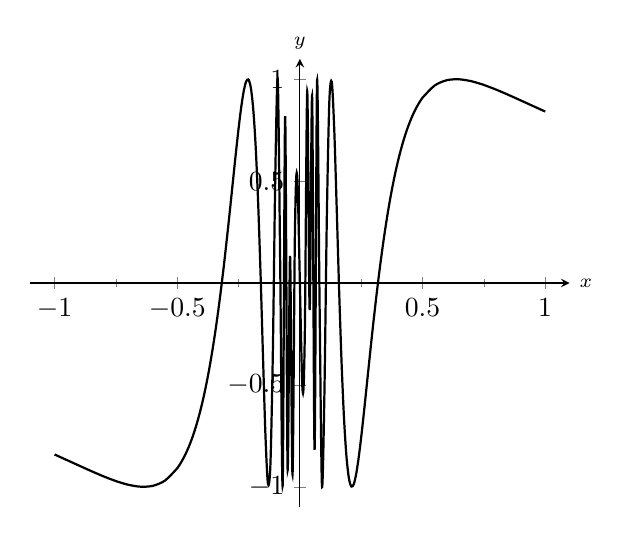
\begin{tikzpicture}
		\begin{axis}[minor x tick num=1,axis y line=middle,axis x line=middle,ymin=-1.1,ymax=1.1,xmin=-1.1,xmax=1.1,name=myplot]
		\addplot [{\colorone},smooth,thick] coordinates {(-1.,-0.841471) (-0.95,-0.86873) (-0.9,-0.896192) (-0.85,-0.923256)(-0.8,-0.948985) (-0.75,-0.971938) (-0.7,-0.989903) (-0.65,-0.999477)(-0.6,-0.995408) (-0.55,-0.969556) (-0.5,-0.909297)(-0.49,-0.891559) (-0.48,-0.871503)(-0.47,-0.848917) (-0.46,-0.823572) (-0.45,-0.79522)(-0.44,-0.763597) (-0.43,-0.728419) (-0.42,-0.689385)(-0.41,-0.64618) (-0.4,-0.598472) (-0.39,-0.545923) (-0.38,-0.488189)(-0.37,-0.424935) (-0.36,-0.355842) (-0.35,-0.280629)(-0.34,-0.199077) (-0.33,-0.11106) (-0.32,-0.0165919)(-0.31,0.0841143) (-0.3,0.190568) (-0.29,0.301898) (-0.28,0.416722)(-0.27,0.532974) (-0.26,0.6477) (-0.25,0.756802) (-0.24,0.854753)(-0.23,0.93428) (-0.22,0.986099) (-0.21,0.998774) (-0.2,0.958924)(-0.19,0.852122) (-0.18,0.665102) (-0.17,0.390185) (-0.16,0.0331792)(-0.15,-0.374151) (-0.14,-0.757628) (-0.13,-0.986959)(-0.12,-0.887294) (-0.11,-0.327701) (-0.1,0.544021) (-0.09,0.993333)(-0.08,0.0663219) (-0.07,-0.988987) (-0.06,0.818447)(-0.05,-0.912945) (-0.04,0.132352) (-0.03,-0.94053) (-0.02,0.262375)(-0.01,0.506366)(0.01,-0.506366) (0.02,-0.262375) (0.03,0.94053) (0.04,-0.132352)(0.05,0.912945) (0.06,-0.818447) (0.07,0.988987) (0.08,-0.0663219)(0.09,-0.993333) (0.1,-0.544021) (0.11,0.327701) (0.12,0.887294)(0.13,0.986959) (0.14,0.757628) (0.15,0.374151) (0.16,-0.0331792)(0.17,-0.390185) (0.18,-0.665102) (0.19,-0.852122) (0.2,-0.958924)(0.21,-0.998774) (0.22,-0.986099) (0.23,-0.93428) (0.24,-0.854753)(0.25,-0.756802) (0.26,-0.6477) (0.27,-0.532974) (0.28,-0.416722)(0.29,-0.301898) (0.3,-0.190568) (0.31,-0.0841143) (0.32,0.0165919)(0.33,0.11106) (0.34,0.199077) (0.35,0.280629) (0.36,0.355842)(0.37,0.424935) (0.38,0.488189) (0.39,0.545923) (0.4,0.598472)(0.41,0.64618) (0.42,0.689385) (0.43,0.728419) (0.44,0.763597)(0.45,0.79522) (0.46,0.823572) (0.47,0.848917) (0.48,0.871503)(0.49,0.891559) (0.5,0.909297)(0.55,0.969556) (0.6,0.995408) (0.65,0.999477) (0.7,0.989903)(0.75,0.971938) (0.8,0.948985) (0.85,0.923256) (0.9,0.896192)(0.95,0.86873) (1.,0.841471) };
		\end{axis}
		\node [right] at (myplot.right of origin) {\scriptsize $x$};
		\node [above] at (myplot.above origin) {\scriptsize $y$};
		\end{tikzpicture}
		\label{fig:nolimit3a}
		\caption{} 
	\end{subfigure}% 
	\begin{subfigure}[t]{0.4\textwidth}
		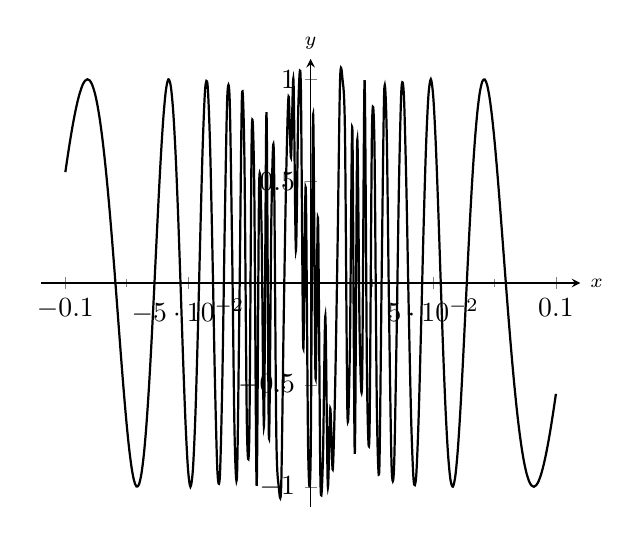
\begin{tikzpicture}
		\begin{axis}[minor x tick num=1,axis y line=middle,axis x line=middle,ymin=-1.1,ymax=1.1,xmin=-.11,xmax=.11,name=myplot]
		\addplot [{\colorone},smooth,thick] coordinates {(-0.1,0.544021) (-0.099,0.625859) (-0.098,0.702784) (-0.097,0.773598) (-0.096,0.837061) (-0.095,0.891904) (-0.094,0.936853) (-0.093,0.970648) (-0.092,0.992071) (-0.091,0.999978) (-0.09,0.993333) (-0.089,0.971247) (-0.088,0.933026) (-0.087,0.878215) (-0.086,0.806651) (-0.085,0.718515) (-0.084,0.614387) (-0.083,0.495298) (-0.082,0.362779) (-0.081,0.218905) (-0.08,0.0663219) (-0.079,-0.0917281) (-0.078,-0.251415) (-0.077,-0.408347) (-0.076,-0.557627) (-0.075,-0.693952) (-0.074,-0.81175) (-0.073,-0.905374) (-0.072,-0.969337) (-0.071,-0.998614) (-0.07,-0.988987) (-0.069,-0.937442) (-0.068,-0.842593) (-0.067,-0.705118) (-0.066,-0.528174) (-0.065,-0.317743) (-0.064,-0.0828681) (-0.063,0.164304) (-0.062,0.408736) (-0.061,0.633044) (-0.06,0.818447) (-0.059,0.94617) (-0.058,0.999301) (-0.057,0.965066) (-0.056,0.837348) (-0.055,0.619211) (-0.054,0.325024) (-0.053,-0.0183676) (-0.052,-0.372047) (-0.051,-0.687679) (-0.05,-0.912945) (-0.049,-0.999926) (-0.048,-0.915928) (-0.047,-0.65528) (-0.046,-0.249359) (-0.045,0.229023) (-0.044,0.671421) (-0.043,0.953507) (-0.042,0.969509) (-0.041,0.67613) (-0.04,0.132352) (-0.039,-0.486679) (-0.038,-0.925763) (-0.037,-0.948132) (-0.036,-0.4764) (-0.035,0.292743) (-0.034,0.907558) (-0.033,0.896983) (-0.032,0.165166) (-0.031,-0.746068) (-0.03,-0.94053) (-0.029,-0.0746909) (-0.028,0.915507) (-0.027,0.614755) (-0.026,-0.690678) (-0.025,-0.745113) (-0.024,0.7352) (-0.023,0.482964) (-0.022,-0.995148) (-0.021,0.475171) (-0.02,0.262375) (-0.019,-0.70007) (-0.018,0.83773) (-0.017,-0.762217) (-0.016,0.325796) (-0.015,0.639018) (-0.014,-0.73662) (-0.013,-0.998945) (-0.012,-0.996711) (-0.011,-0.195822) (-0.01,0.506366) (-0.009,0.914944) (-0.008,0.61604) (-0.007,0.996362) (-0.006,0.161545) (-0.005,0.873297) (-0.004,0.970528) (-0.003,-0.318846) (-0.002,0.467772) (-0.001,-0.82688) (0,-0.85773) (0.001,0.82688) (0.002,-0.467772) (0.003,0.318846) (0.004,-0.970528) (0.005,-0.873297) (0.006,-0.161545) (0.007,-0.996362) (0.008,-0.61604) (0.009,-0.914944) (0.01,-0.506366) (0.011,0.195822) (0.012,0.996711) (0.013,0.998945) (0.014,0.73662) (0.015,-0.639018) (0.016,-0.325796) (0.017,0.762217) (0.018,-0.83773) (0.019,0.70007) (0.02,-0.262375) (0.021,-0.475171) (0.022,0.995148) (0.023,-0.482964) (0.024,-0.7352) (0.025,0.745113) (0.026,0.690678) (0.027,-0.614755) (0.028,-0.915507) (0.029,0.0746909) (0.03,0.94053) (0.031,0.746068) (0.032,-0.165166) (0.033,-0.896983) (0.034,-0.907558) (0.035,-0.292743) (0.036,0.4764) (0.037,0.948132) (0.038,0.925763) (0.039,0.486679) (0.04,-0.132352) (0.041,-0.67613) (0.042,-0.969509) (0.043,-0.953507) (0.044,-0.671421) (0.045,-0.229023) (0.046,0.249359) (0.047,0.65528) (0.048,0.915928) (0.049,0.999926) (0.05,0.912945) (0.051,0.687679) (0.052,0.372047) (0.053,0.0183676) (0.054,-0.325024) (0.055,-0.619211) (0.056,-0.837348) (0.057,-0.965066) (0.058,-0.999301) (0.059,-0.94617) (0.06,-0.818447) (0.061,-0.633044) (0.062,-0.408736) (0.063,-0.164304) (0.064,0.0828681) (0.065,0.317743) (0.066,0.528174) (0.067,0.705118) (0.068,0.842593) (0.069,0.937442) (0.07,0.988987) (0.071,0.998614) (0.072,0.969337) (0.073,0.905374) (0.074,0.81175) (0.075,0.693952) (0.076,0.557627) (0.077,0.408347) (0.078,0.251415) (0.079,0.0917281) (0.08,-0.0663219) (0.081,-0.218905) (0.082,-0.362779) (0.083,-0.495298) (0.084,-0.614387) (0.085,-0.718515) (0.086,-0.806651) (0.087,-0.878215) (0.088,-0.933026) (0.089,-0.971247) (0.09,-0.993333) (0.091,-0.999978) (0.092,-0.992071) (0.093,-0.970648) (0.094,-0.936853) (0.095,-0.891904) (0.096,-0.837061) (0.097,-0.773598) (0.098,-0.702784) (0.099,-0.625859) (0.1,-0.544021)
		};
		\end{axis}
		\node [right] at (myplot.right of origin) {\scriptsize $x$};
		\node [above] at (myplot.above origin) {\scriptsize $y$};
		\end{tikzpicture}
		\label{fig:nolimit3b}
		\caption{}    
	\end{subfigure} 
	\begin{subfigure}[t]{0.2\textwidth}
					\begin{tabular}{cc}
						0.1 & -0.544021 \\
						0.01 & -0.506366 \\
						0.001 & 0.82688 \\
						0.0001 & -0.305614 \\
						1$\times 10^{-5}$ & 0.0357488 \\
						1$\times 10^{-6}$& -0.349994\\
						1$\times 10^{-7}$ & 0.420548
					\end{tabular}
		\label{fig:nolimit3c}
		\caption{}    
	\end{subfigure} 
	\caption{Observing that $f(x) = \sin(1/x)$ has no limit as $x\to 0$ \label{fig:nolimit3} }
\end{figure}



\subsection{Limits of Difference Quotients}\label{subsec:limitofdiffquotientintro}
%
We have approximated limits of functions as $x$ approached a particular number. We will consider another important kind of limit after explaining a few key ideas.\index{limit!difference quotient}

\mfigure{.5}{Interpreting a difference quotient as the slope of a secant line.}{fig:diffquot1}{ %
\begin{tikzpicture}
\begin{axis}[clip=false, minor x tick num=1,axis y line=middle,axis x line=middle,ymin=-1,ymax=25,extra y tick labels={},xmin=-1,xmax=6.5,name=myplot]
\addplot [{\colorone},smooth,thick] coordinates {(0.,0.) (0.5,5.375) (1.,10.) (1.5,13.875) (2.,17.) (2.5,19.375)(3.,21.) (3.5,21.875) (4.,22.) (4.5,21.375) (5.,20.) (5.5,17.875)(6.,15.) };
\addplot [{\colortwo},smooth,thick] coordinates {(0,7.5) (6,22.5)};
\fill[black] (axis cs:1,10) circle (1pt);
\fill[black] (axis cs:5,20) circle (1pt);
\end{axis}
\node [right] at (myplot.right of origin) { $x$};
\node [above] at (myplot.above origin) { $f$};
\end{tikzpicture}
}

Let $f(x)$ represent the position function, in feet, of some particle that is moving in a straight line, where $x$ is measured in seconds. Let's say that when $x=1$, the particle is at position 10 ft., and when $x=5$, the particle is at 20 ft. Another way of expressing this is to say $$f(1)=10 \quad \text{ and } \quad f(5) = 20.$$
Since the particle traveled 10 feet in 4 seconds, we can say the particle's \textit{average velocity} was 2.5 ft/s. We write this calculation using a ``quotient of differences,'' or, a \textit{difference quotient}: $$\frac{f(5) - f(1)}{5-1} = \frac{10}4 = 2.5 \text{ft/s}.$$

This difference quotient can be thought of as the familiar ``rise over run'' used to compute the slopes of lines. In fact, that is essentially what we are doing: given two points on the graph of $f$, we are finding the slope of the \textit{secant line} through those two points. See Figure \ref{fig:diffquot1}.

Now consider finding the average speed on another time interval. We again start at $x=1$, but consider the position of the particle $h$ seconds later. That is, consider the positions of the particle when $x=1$ and when $x=1+h$. The difference quotient is now $$\frac{f(1+h)-f(1)}{(1+h)-1} = \frac{f(1+h)-f(1)}h.$$

Let $f(x) = -1.5x^2+11.5x$; note that $f(1)=10$ and $f(5) = 20$, as in our discussion. We can compute this difference quotient for all values of $h$ (even negative values!) except $h=0$, for then we get ``0/0,'' the indeterminate form introduced earlier. For all values $h\neq 0$, the difference quotient computes the average velocity of the particle over an interval of time of length $h$ starting at $x=1$. 

For small values of $h$, i.e., values of $h$ close to $ 0 $, we get average velocities over very short time periods and compute secant lines over small intervals. See Figure \ref{fig:diff_quot_small_h}. This leads us to wonder what the limit of the difference quotient is as $h$ approaches $ 0 $. That is, $$\lim_{h\to 0} \frac{f(1+h)-f(1)}{h} = \text{ ? }$$

\begin{figure}
	\centering
	\begin{subfigure}[t]{0.33\textwidth}
		 \begin{tikzpicture}
		 \begin{axis}[clip=false,minor x tick num=1,axis y line=middle,axis x line=middle,ymin=-1,ymax=25,extra y tick labels={},xmin=-1,xmax=6.5,name=myplot]
		 \addplot [{\colorone},smooth,thick] coordinates {(0.,0.) (0.5,5.375) (1.,10.) (1.5,13.875) (2.,17.) (2.5,19.375)(3.,21.) (3.5,21.875) (4.,22.) (4.5,21.375) (5.,20.) (5.5,17.875)(6.,15.) };
		 \addplot [{\colortwo},smooth,thick] coordinates {(0,4.5) (4,26.5)};
		 \fill[black] (axis cs:1,10) circle (1pt);
		 \fill[black] (axis cs:3,21) circle (1pt);
		 \end{axis}
		 \node [right] at (myplot.right of origin) { $x$};
		 \node [above] at (myplot.above origin) { $f$};
		 \end{tikzpicture}
        \label{fig:diff_quot_small_ha}
        \caption{$ h=2 $} 
    \end{subfigure}% 
    \begin{subfigure}[t]{0.33\textwidth}
     \begin{tikzpicture}
     \begin{axis}[clip=false,tick label style={font=\scriptsize},minor x tick num=1,axis y line=middle,axis x line=middle,ymin=-1,ymax=25,extra y tick labels={},xmin=-1,xmax=6.5,name=myplot]
     \addplot [{\colorone},smooth,thick] coordinates {(0.,0.) (0.5,5.375) (1.,10.) (1.5,13.875) (2.,17.) (2.5,19.375)(3.,21.) (3.5,21.875) (4.,22.) (4.5,21.375) (5.,20.) (5.5,17.875)(6.,15.) };
     \addplot [{\colortwo},smooth,thick] coordinates {(0,3) (3,24)};
     \fill[black] (axis cs:1,10) circle (1pt);
     \fill[black] (axis cs:2,17) circle (1pt);
     \end{axis}
     \node [right] at (myplot.right of origin) {$x$};
     \node [above] at (myplot.above origin) { $f$};
     \end{tikzpicture}
        \label{fig:diff_quot_small_hb}
        \caption{$ h=1 $}    
    \end{subfigure}
\begin{subfigure}[t]{0.33\textwidth}
     \begin{tikzpicture}
     \begin{axis}[clip=false,minor x tick num=1,axis y line=middle,axis x line=middle,ymin=-1,ymax=25,extra y tick labels={},xmin=-1,xmax=6.5,name=myplot]
     \addplot [{\colorone},smooth,thick] coordinates {(0.,0.) (0.5,5.375) (1.,10.) (1.5,13.875) (2.,17.) (2.5,19.375)(3.,21.) (3.5,21.875) (4.,22.) (4.5,21.375) (5.,20.) (5.5,17.875)(6.,15.) };
     \addplot [{\colortwo},smooth,thick] coordinates {(0,2.25) (2.5,21.625)};
     \fill[black] (axis cs:1,10) circle (1pt);
     \fill[black] (axis cs:1.5,13.875) circle (1pt);
     \end{axis}
     \node [right] at (myplot.right of origin) { $x$};
     \node [above] at (myplot.above origin) {$f$};
     \end{tikzpicture}
        \label{fig:diff_quot_small_hc}
        \caption{$ h=.5 $}    
    \end{subfigure} 
    \caption{Secant lines of $f(x)$ at $x=1$ and $x=1+h$, for shrinking values of $h$ (i.e., $h\rightarrow 0$).\label{fig:diff_quot_small_h} }
\end{figure}



As we do not yet have a true definition of a limit nor an exact method for computing it, we settle for approximating the value. While we could graph the difference quotient (where the $x$-axis would represent $h$ values and the $y$-axis would represent values of the difference quotient) we settle for making a table. See Figure \ref{table:diff_quot_smallh}. The table gives us reason to assume the value of the limit is about 8.5. \\

\mTable{.5}{The difference quotient evaluated at values of $h$ near 0.}{table:diff_quot_smallh}{\begin{tabular}{cc}$h$ & $\frac{f(1+h)-f(1)}{h}$\vspace{1pt} \\ \hline $-0.5$ & 9.25 \\ $-0.1$ & 8.65 \\ $-0.01$ & 8.515 \\ 0.01 & 8.485 \\ 0.1 & 8.35 \\ 0.5 & 7.75 \end{tabular}} 




% % % % % % % % % % % % % % % % % % % % % % % % % % % % % % % % % % % % % % % % % % % % % % % % % % % %
\subsection*{One-sided limits}
Consider the following piecewise defined function:
%$$f(x)=
%\left\{\begin{array}{ccc}
%x,&\quad&\mbox{if $x\leq 1$,}\\
%x+1,&\quad&\mbox{if $x>1$,}\\
%\end{array}\right.$$
%which has the following visual representation:
$$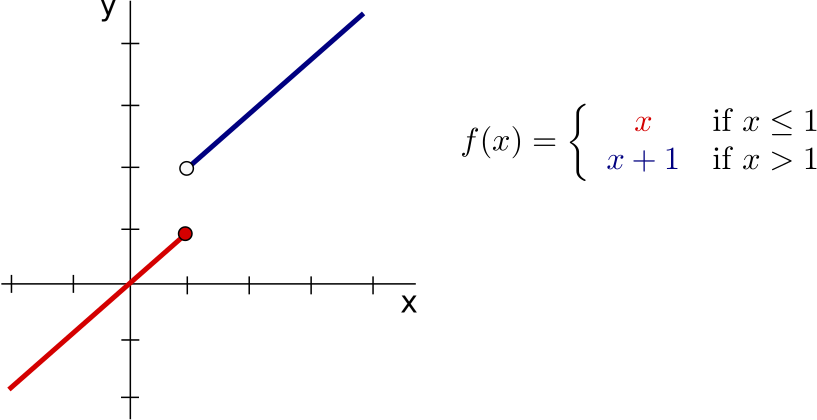
\includegraphics[width=4.0in]{images/limits-1}$$ Observe from the
graph that as $x$ gets closer and closer to $1$ from the \textit{left},
then $f(x)$ approaches $+1$.  Similarly, as $x$ gets closer and closer
$1$ from the \textit{right}, then $f(x)$ approaches $+2$.  We use the
following notation to indicate this: $$\lim_{x\to
1^-}f(x)=1\qquad\mbox{and}\qquad\lim_{x\to 1^+}f(x)=2.$$ 
%The symbol
%$x\to 1^-$ means that we only consider values of $x$ sufficiently
%close to $1$ which are less than $1$.  Similarly, the symbol $x\to
%1^+$ means that we only consider values of $x$ sufficiently close to
%$1$ which are greater than $1$.

\begin{definition}{Left and Right-Hand Limit (Useable Definition)}{LeftRightHandLimit}
In general, we will write
$$\lim_{x\to a^-}f(x)=L,$$
if we can make the values of $f(x)$ arbitrarily close to $L$ by taking $x$ to be sufficiently close to $a$ and $x$ less than $a$.
This is called the {\textbf{left-hand limit}} of $f(x)$ as $x$ approaches $a$.
Similarly, we write
$$\lim_{x\to a^+}f(x)=L,$$
if we can make the values of $f(x)$ arbitrarily close to $L$ by taking $x$ to be sufficiently close to $a$ and $x$ greater than $a$.
This is called the  {\textbf{right-hand limit}} of $f(x)$ as $x$ approaches $a$.
\end{definition}



Practically speaking, when evaluating a left-hand limit at $ a $, we consider only values of $x$ ``to the left of $a$,'' on the real number line i.e., where $x<a$. The admittedly imperfect notation $x\to a^-$ is used to imply that we look at values of $x$ to the left of $a$. The notation has nothing to do with positive or negative values of either $x$ or $a$. A similar statement holds for evaluating right-hand limits; there we consider only values of $x$ to the right of $a$ on the real number line, i.e., $x>a$. 

%We can use the theorems from previous sections to help us evaluate these limits; we just restrict our view to one side of $c$.

We practice evaluating left and right-hand limits through a series of examples.\\


\begin{example}{Evaluating one sided limits}{ex_onesidea}{
Let $\ds f(x) = \left\{\begin{array}{cc} x & 0\leq x\leq 1 \\ 3-x & 1<x<2\end{array},\right.$ as shown in Figure \ref{fig:onesided1}. Find each of the following: 

\noindent\begin{minipage}[t]{.5\textwidth}
\begin{enumerate}
\item		$\ds \lim_{x\to 1^-} f(x)$
\item		$\ds \lim_{x\to 1^+} f(x)$
\item		$\ds \lim_{x\to 1} f(x)$
\item		$\ds f(1)$
\end{enumerate}
\end{minipage}
\begin{minipage}[t]{.5\textwidth}
\begin{enumerate}\addtocounter{enumi}{4}
\item		$\ds \lim_{x\to 0^+} f(x)$
\item		$f(0)$
\item		$\ds \lim_{x\to 2^-} f(x)$
\item		$f(2)$
\end{enumerate}
\end{minipage}

\mfigure{.65}{A graph of $f$ in Example \ref{exa:ex_onesidea}.}{fig:onesided1}{\centering \begin{tikzpicture}
\begin{axis}[minor x tick num=1,axis y line=middle,axis x line=middle,ymin=-.4,ymax=2.4,xmin=-.4,xmax=2.4,name=myplot]
\addplot [{\colorone},smooth,thick] coordinates {(0,0) (1,1)};
\fill[black,draw=black] (axis cs:1,1) circle (1.5pt);
\fill[black,draw=black] (axis cs:0,0) circle (1.5pt);
\addplot [{\colorone},smooth,thick] coordinates {(1,2) (2,1)};
\fill[white,draw=black,thick] (axis cs:1,2) circle (1.5pt);
\fill[white,draw=black,thick] (axis cs:2,1) circle (1.5pt);
\end{axis}
\node [right] at (myplot.right of origin) {  $x$};
\node [above] at (myplot.above origin) {  $y$};
\end{tikzpicture}
% this is the sqrt[x] on [0,5]} %
}
}
\end{example}


\begin{solution}
{For these problems, the visual aid of the graph effective in evaluating the limits.
			\begin{enumerate}
			\item		As $x$ goes to 1 \textit{from the left}, we see that $f(x)$ is approaching the value of 1. Therefore $\ds \lim_{x\to 1^-} f(x) =1.$
			\item		As $x$ goes to 1 \textit{from the right}, we see that $f(x)$ is approaching the value of 2. Recall that it does not matter that there is an ``open circle'' there; we are evaluating a limit, not the value of the function. Therefore $\ds \lim_{x\to 1^+} f(x)=2$.
			\item		\textit{The} limit of $f$ as $x$ approaches 1 does not exist since the function does not approach one particular value, but two different values from the left and the right.
			\item		Using the definition and by looking at the graph we see that $f(1) = 1$.
			\item		As $x$ goes to 0 from the right, we see that $f(x)$ is also approaching 0. Therefore $\ds \lim_{x\to 0^+} f(x)=0$. Note we cannot consider a left-hand limit at 0 as $f$ is not defined for values of $x<0$.
			\item		Using the definition and the graph, $f(0) = 0$.
			\item		As $x$ goes to 2 from the left, we see that $f(x)$ is approaching the value of 1. Therefore $\ds \lim_{x\to 2^-} f(x)=1.$
			\item		The graph and the definition of the function show that $f(2)$ is not defined.
			\end{enumerate}
}
\end{solution}






%We note the following fact:
%\begin{center}
%$\ds{\lim_{x\to a}f(x)=L\qquad\mbox{if and only if}\qquad\lim_{x\to a^-}f(x)=L\qquad\mbox{and}\qquad\lim_{x\to a^+}f(x)=L}.$
%\end{center}
%Or more concisely:
%\[\lim_{x\to a^-}f(x)=\lim_{x\to a^+}f(x)=L\].
%A consequence of this fact is that if the one-sided limits are \ifont{different}, then the two-sided limit $\ds{\lim_{x\to a}f(x)}$ does not exist, often denoted as: (DNE).


Note how the left and right-hand limits were different at $x=1$. This, of course, causes \textit{the} limit to not exist. The following theorem states what is fairly intuitive: \textit{the} limit exists precisely when the left and right-hand limits are equal.

\begin{theorem}{Limits and One Sided Limits}{leftrightlimits}
{Let $f$ be a function defined on an open interval $I$ containing $c$. \index{limit!does not exist} Then $$\lim_{x\to c}f(x) = L$$ if, and only if, $$\lim_{x\to c^-}f(x) = L \quad \text{and} \quad \lim_{x\to c^+}f(x) = L.$$}
\end{theorem}

The phrase ``if, and only if'' means the two statements are \textit{equivalent}: they are either both true or both false. If the limit equals $L$, then the left and right hand limits both equal $L$. If the limit is not equal to $L$, then at least one of the left and right-hand limits is not equal to $L$ (it may not even exist).
			
One thing to consider in Examples \ref{exa:ex_onesidea} -- \ref{exa:ex_onesided} is that the value of the function may/may not be equal to the value(s) of its left/right-hand limits, even when these limits agree. \\


\begin{example}{Evaluating limits of a piecewise--defined function}{ex_onesideb}{
Let $f(x) = \left\{\begin{array}{cc} 2-x & 0<x<1 \\ (x-2)^2 & 1<x<2 \end{array},\right.$ as shown in Figure \ref{fig:onesidedb}. Evaluate the following. 

\noindent\begin{minipage}[t]{.5\textwidth}
		\begin{enumerate}
		\item		$\ds \lim_{x\to 1^-} f(x)$
		\item		$\ds \lim_{x\to 1^+} f(x)$
		\item		$\ds \lim_{x\to 1} f(x)$
		\item		$\ds f(1)$
		\end{enumerate}
		\end{minipage}
		\begin{minipage}[t]{.5\textwidth}
		\begin{enumerate}\addtocounter{enumi}{4}
		\item		$\ds \lim_{x\to 0^+} f(x)$
		\item		$f(0)$
		\item		$\ds \lim_{x\to 2^-} f(x)$
		\item		$f(2)$
		\end{enumerate}	
		\end{minipage}
		
\mfigure{.7}{A graph of $f$ from Example \ref{exa:ex_onesideb}}{fig:onesidedb}{ %
\begin{tikzpicture}
\begin{axis}[minor x tick num=1,axis y line=middle,axis x line=middle,ymin=-.4,ymax=2.4,xmin=-.4,xmax=2.4,name=myplot]
\addplot [{\colorone},smooth,thick] coordinates {(0,2) (1,1)};
\addplot [{\colorone},smooth,thick] coordinates {(1.,1.) (1.1,0.81) (1.2,0.64) (1.3,0.49) (1.4,0.36) (1.5,0.25) (1.6,0.16) (1.7,0.09) (1.8,0.04) (1.9,0.01) (2.,0.)};
\fill[white,draw=black,thick] (axis cs:2,0) circle (1.5pt);
\fill[white,draw=black,thick] (axis cs:0,2) circle (1.5pt);
\fill[white,draw=black,thick] (axis cs:1,1) circle (1.5pt);
%\fill[white,draw=black] (axis cs:2,1) circle (1pt);
\end{axis}
\node [right] at (myplot.right of origin) { $x$};
\node [above] at (myplot.above origin) {  $y$};
\end{tikzpicture}
}		
}
\end{example}


\begin{solution}
{Again we will evaluate each using both the definition of $f$ and its graph.
		\begin{enumerate}
		\item		As $x$ approaches $ 1 $ from the left, we see that $f(x)$ approaches $ 1 $. Therefore $\ds \lim_{x\to 1^-} f(x)=1.$
		\item		As $x$ approaches 1 from the right, we see that again $f(x)$ approaches 1. Therefore $\ds \lim_{x\to 1+} f(x)=1$.
		\item		\textit{The} limit of $f$ as $x$ approaches 1 exists and is 1, as $f$ approaches 1 from both the right and left. Therefore $\ds \lim_{x\to 1} f(x)=1$.
		\item		$f(1)$ is not defined. Note that 1 is not in the domain of $f$ as defined by the problem, which is indicated on the graph by an open circle when $x=1$.
		\item		As $x$ goes to 0 from the right, $f(x)$ approaches 2. So $\ds \lim_{x\to 0^+} f(x)=2$.
		\item		$f(0)$  is not defined as $0$ is not in the domain of $f$.
		\item		As $x$ goes to 2 from the left, $f(x)$ approaches 0. So $\ds \lim_{x\to 2^-} f(x)=0$.
		\item		$f(2)$  is not defined as 2 is not in the domain of $f$.
		\end{enumerate}
}
\end{solution}





%
\begin{example}{Evaluating limits of a piecewise--defined function}{ex_onesidec}{
Let $f(x) = \left\{\begin{array}{cc} (x-1)^2 & 0\leq x\leq 2, x\neq 1\\ 1 & x=1\end{array},\right.$ as shown in Figure \ref{fig:onesidedc}. Evaluate the following.

		\noindent\begin{minipage}[t]{.5\textwidth}
		\begin{enumerate}
		\item		$\ds \lim_{x\to 1^-} f(x)$
		\item		$\ds \lim_{x\to 1^+} f(x)$
		\end{enumerate}
		\end{minipage}
		\begin{minipage}[t]{.5\textwidth}
		\begin{enumerate}\addtocounter{enumi}{2}
		\item		$\ds \lim_{x\to 1} f(x)$
		\item		$f(1)$
		\end{enumerate}
		\end{minipage}
		
\mfigure{.7}{Graphing $f$ in Example \ref{exa:ex_onesidec}}{fig:onesidedc}{ %
\begin{tikzpicture}
\begin{axis}[minor x tick num=1,axis y line=middle,axis x line=middle,ymin=-.4,ymax=1.4,xmin=-.4,xmax=2.4,name=myplot]
%\addplot [{\colorone},smooth] coordinates {(0,2) (1,1)};
\addplot [{\colorone},smooth,thick] coordinates {(0.,1.) (0.1,0.81) (0.2,0.64) (0.3,0.49) (0.4,0.36) (0.5,0.25) (0.6,0.16) (0.7,0.09) (0.8,0.04) (0.9,0.01) (1.,0.) (1.1,0.01)
(1.2,0.04) (1.3,0.09) (1.4,0.16) (1.5,0.25) (1.6,0.36) (1.7,0.49)
(1.8,0.64) (1.9,0.81) (2.,1.)
};
\fill[black,draw=black] (axis cs:0,1) circle (1.5pt);
\fill[black,draw=black] (axis cs:2,1) circle (1.5pt);
\fill[black,draw=black] (axis cs:1,1) circle (1.5pt);
\fill[white,draw=black,thick] (axis cs:1,0) circle (1.5pt);
\end{axis}
\node [right] at (myplot.right of origin) { $x$};
\node [above] at (myplot.above origin) { $y$};
\end{tikzpicture}}		
}
\end{example}


\begin{solution}
{		It is clear by looking at the graph that both the left and right-hand limits of $f$, as $x$ approaches 1, is 0. Thus it is also clear that \textit{the} limit is 0; i.e., $\ds \lim_{x\to 1} f(x) = 0$. It is also clearly stated that $f(1) = 1$. \vskip .4\baselineskip
}
\end{solution}





\begin{example}{Evaluating limits of a piecewise--defined function}{ex_onesided}{
Let $f(x) = \left\{\begin{array}{cc} x^2 & 0\leq x\leq 1 \\ 2-x & 1<x\leq 2\end{array},\right.$ as shown in Figure \ref{fig:onesidedd}. Evaluate the following. 

		\noindent\begin{minipage}[t]{.5\textwidth}
		\begin{enumerate}
		\item		$\ds \lim_{x\to 1^-} f(x)$
		\item		$\ds \lim_{x\to 1^+} f(x)$
		\end{enumerate}
		\end{minipage}
				\noindent\begin{minipage}[t]{.5\textwidth}
		\begin{enumerate}\addtocounter{enumi}{2}
		\item		$\ds \lim_{x\to 1} f(x)$
		\item		$f(1)$
		\end{enumerate}
		\end{minipage}		
}
%\mfigure{.7}{Graphing $f$ in Example \ref{exa:ex_onesided}}{fig:onesided}{ %

\end{example}


\begin{solution}
{		It is clear from the definition of the function and its graph that all of the following are equal:
\mfigure{.8}{Graphing $f$ in Example \ref{exa:ex_onesided}}{fig:onesidedd}{\begin{tikzpicture}
\begin{axis}[minor x tick num=1,axis y line=middle,axis x line=middle,ymin=-.4,ymax=1.4,xmin=-.4,xmax=2.4,name=myplot]
\addplot [{\colorone},smooth,thick] coordinates {(2,0) (1,1)};
\addplot [{\colorone},smooth,thick] coordinates {(0.,0.) (0.1,0.01) (0.2,0.04) (0.3,0.09) (0.4,0.16) (0.5,0.25)(0.6,0.36) (0.7,0.49) (0.8,0.64) (0.9,0.81) (1.,1.) };
\fill[black,draw=black] (axis cs:0,0) circle (1.5pt);
\fill[black,draw=black] (axis cs:1,1) circle (1.5pt);
\fill[black,draw=black] (axis cs:2,0) circle (1.5pt);
%\fill[white,draw=black] (axis cs:2,1) circle (1pt);
\end{axis}
\node [right] at (myplot.right of origin) {  $x$};
\node [above] at (myplot.above origin) {  $y$};
\end{tikzpicture}}
$$ \lim_{x\to 1^-} f(x) = \lim_{x\to 1^+} f(x) =\lim_{x\to 1} f(x) =f(1) = 1.$$
}
\end{solution}







In Examples \ref{ex_onesidea} -- \ref{ex_onesided} we were asked to find both $\ds \lim_{x\to 1}f(x)$ and $f(1)$. Consider the following table:
\begin{center}
\begin{tabular}{ccc} & $\ds \lim_{x\to 1}f(x)$ & $f(1)$ \vspace{2pt}\\ \hline
Example \ref{exa:ex_onesidea} & does not exist & 1 \\
Example \ref{exa:ex_onesideb} & 1 & not defined \\
Example \ref{exa:ex_onesidec} & 0 & 1 \\
Example \ref{exa:ex_onesided} & 1 & 1 \\
\end{tabular}
\end{center}

Only in Example \ref{exa:ex_onesided} do both the function and the limit exist and agree. This seems ``nice;'' in fact, it seems ``normal.'' This is in fact an important situation which we explore in the next section, entitled ``Continuity.'' In short, a \textit{continuous function} is one in which when a function approaches a value as $x\rightarrow c$ (i.e., when $\ds \lim_{x\to c} f(x) = L$), it actually \textit{attains} that value at $c$. Such functions behave nicely as they are very predictable.



Proper understanding of limits is key to understanding calculus. With limits, we can accomplish seemingly impossible mathematical things, like adding up an infinite number of numbers (and not get infinity) and finding the slope of a line between two points, where the ``two points'' are actually the same point. These are not just mathematical curiosities; they allow us to link position, velocity and acceleration together, connect cross-sectional areas to volume, find the work done by a variable force, and much more.


In the next section we give the formal definition of the limit and begin our study of finding limits analytically. 









%In the following exercises, we continue our introduction and approximate the value of limits.\\
%
%\printexercises{exercises/01_01_exercises}


%One-sides:
%
%\printexercises{exercises/01_04_exercises}


%%%%%%%%%%%%%%%%%%%%%%%%%%%%%%%%%%%%%%%%%%%%
\Opensolutionfile{solutions}[ex]
\section*{Exercises for Section \ref{sec:LimitsWorkingDefn}}

\begin{multicols}{2}

\begin{enumialphparenastyle}

%%%%%%%%%%
% % % % % % % % % % %
\begin{ex}
\begin{enumerate}
\item {In your own words, what does it mean to ``find the limit of $f(x)$ as $x$ approaches 3''?}

\item {An expression of the form $\frac00$ is called \underline{\hskip 15pt}.}

\item {T/F: The limit of $f(x)$ as $x$ approaches $5$ is $f(5)$.}

\item {Describe three situations where $\displaystyle \lim_{x\to c}f(x)$ does not exist.}

\item {In your own words, what is a difference quotient?}

\item {T/F: If $\ds \lim_{x\to 1^-} f(x) = 5$, then $\ds \lim_{x\to 1} f(x) = 5$}

\item {T/F: If $\ds \lim_{x\to 1^-} f(x) = 5$, then $\ds \lim_{x\to 1^+} f(x) = 5$}

\item {T/F: If $\ds \lim_{x\to 1} f(x) = 5$, then $\ds \lim_{x\to 1^-} f(x) = 5$}

\end{enumerate}

\begin{sol}
\begin{enumerate}
\item {Answers will vary.}
\item {An indeterminate form.}
\item {F}
\item {The function may approach different values from the left and right, the function may grow without bound, or the function might oscillate.}
\item {Answers will vary.}
\item {F}
\item {F}
\item {T}
\end{enumerate}
\end{sol}

\end{ex}
% % % % % % % % % % % %
\begin{ex}
Evaluate the expressions by reference to this graph:
$$\includegraphics[width=3.5in]{images/limit-exercise-graph}$$
\begin{multicols}{3}
\begin{enumerate}
	\item	$\ds \lim_{x\to 4} f(x)$
	\item	$\ds \lim_{x\to -3} f(x)$
	\item	$\ds \lim_{x\to 0} f(x)$
	\item	$\ds \lim_{x\to 0^-} f(x)$
	\item	$\ds \lim_{x\to 0^+} f(x)$
	\item	$\ds f(-2)$
	\item	$\ds \lim_{x\to 2^-} f(x)$
	\item	$\ds \lim_{x\to -2^-} f(x)$
	\item	$\ds \lim_{x\to 0} f(x+1)$
	\item	$\ds f(0)$
	\item	$\ds \lim_{x\to 1^-} f(x-4)$
	\item	$\ds \lim_{x\to 0^+} f(x-2)$
\end{enumerate}
\end{multicols}
\begin{sol}
\begin{multicols}{3}
\begin{enumerate}
	\item	$8$
	\item	$6$
	\item	dne
	\item	$-2$
	\item	$-1$
	\item	$8$
	\item	$7$
	\item	$6$
	\item	$3$
	\item	$-3/2$
	\item	$6$
	\item	$2$
\end{enumerate}
\end{multicols}
\end{sol}
\end{ex}

% % % % % % % % % % %
\begin{ex}
Approximate the given limits both numerically and graphically.
\begin{enumerate}
\item {$-1$}
\item {$\displaystyle \lim_{x\to 0} x^3-3x^2+x-5$}
\item {$\displaystyle \lim_{x\to 0} \frac{x+1}{x^2+3x}$}
\item {$\displaystyle \lim_{x\to 3} \frac{x^2-2x-3}{x^2-4x+3}$}
\item {$\displaystyle \lim_{x\to -1} \frac{x^2+8x+7}{x^2+6x+5}$}
\item {$\displaystyle \lim_{x\to 2} \frac{x^2+7x+10}{x^2-4x+4}$}
\item {$\displaystyle \lim_{x\to 2} f(x)$, where 

$f(x) = \left\{\begin{array}{cl} x+2 & x\leq 2 \\ 3x-5 & x>2 \end{array}\right.$.
}
\item {$\displaystyle \lim_{x\to 3} f(x)$, where 

$f(x) = \left\{\begin{array}{cl} x^2-x+1 & x\leq 3 \\ 2x+1 & x>3 \end{array}\right.$.}
\item {$\displaystyle \lim_{x\to 0} f(x)$, where 

$f(x) = \left\{\begin{array}{cl} \cos x & x\leq 0 \\ x^2+3x+1 & x>0 \end{array}\right.$.}
\item  {$\displaystyle \lim_{x\to \pi/2} f(x)$, where 

$f(x) = \left\{\begin{array}{cl} \sin x & x\leq \pi/2 \\ \cos x & x>\pi/2 \end{array}\right.$.}
\end{enumerate}

\begin{sol}
\begin{enumerate}
\item {$\displaystyle \lim_{x\to 1} x^2+3x-5$}
\item {$-5$}
\item {Limit does not exist}
\item  {$2$}
\item {$1.5$}
\item 
{Limit does not exist.}
\item 
{Limit does not exist.}
\item 
{$7$}
\item 
{$1$}
\item 
{Limit does not exist.}

\end{enumerate}
\end{sol}

\end{ex}
% % % % % % % % % % % %

% % % % % % % % % % %
\begin{ex}
A function $f$ and a value $a$ are given. Approximate the limit of the difference quotient, $\displaystyle \lim_{h\to 0}\frac{f(a+h)-f(a)}{h}$, using $h = \pm 0.1, \pm 0.01$.
\begin{enumerate}
\item {$f(x) = -7x+2$,\quad  $a=3$}
\item {$f(x) = 9x+0.06$,\quad  $a=-1$}
\item {$f(x) = x^2+3x-7$,\quad  $a=1$}
\item {$\displaystyle f(x) = \frac{1}{x+1}$,\quad  $a=2$}
\item {$\displaystyle f(x) = -4x^2+5x-1$,\quad  $a=-3$}
\item {$\displaystyle f(x) =\ln x$,\quad  $a=5$}
\item {$\displaystyle f(x) =\sin x$,\quad $a=\pi$} 
\item {$\displaystyle f(x) =\cos x$,\quad  $a=\pi$}

\end{enumerate}

\begin{sol}
\begin{enumerate}
\item 
{\begin{tabular}{cc}
$h$ & $\frac{f(a+h)-f(a)}{h}$\\ \hline 
 $-0.1$ & $-7$ \\
 $-0.01$ & $-7$ \\
 $0.01$ & $-7$ \\
 $0.1$ & $-7$
\end{tabular}
The limit seems to be exactly 7.
}
\item 
{\begin{tabular}{cc}
$h$ & $\frac{f(a+h)-f(a)}{h}$\\ \hline 
 $-0.1$ & $9$ \\
 $-0.01$ & $9$ \\
 $0.01$ & $9$ \\
 $0.1$ & $9$
\end{tabular}
The limit seems to be exactly 9.
}
\item 
{\begin{tabular}{cc}
$h$ & $\frac{f(a+h)-f(a)}{h}$\\ \hline 
 $-0.1$ & $4.9$ \\
 $-0.01$ & $4.99$ \\
 $0.01$ & $5.01$ \\
 $0.1$ & $5.1$
\end{tabular}
The limit is approx. 5.
}
\item 
{\begin{tabular}{cc}
$h$ & $\frac{f(a+h)-f(a)}{h}$\\ \hline
 $-0.1$ & $-0.114943$ \\
 $-0.01$ & $-0.111483$ \\
 $0.01$ & $-0.110742$ \\
 $0.1$ & $-0.107527$
\end{tabular}
The limit is approx. $-0.11$.
}
\item 
{\begin{tabular}{cc}
$h$ & $\frac{f(a+h)-f(a)}{h}$\\ \hline 
 $-0.1$ & $29.4$ \\
 $-0.01$ & $29.04$ \\
 $0.01$ & $28.96$ \\
 $0.1$ & $28.6$
\end{tabular}
The limit is approx. $29$.
}
\item 
{\begin{tabular}{cc}
$h$ & $\frac{f(a+h)-f(a)}{h}$\\ \hline
 $ -0.1$ & $0.202027$ \\
 $-0.01$ & $0.2002$ \\
 $0.01$ & $0.1998$ \\
 $0.1$ & $0.198026$
\end{tabular}
The limit is approx. $0.2$.
}
\item 
{\begin{tabular}{cc}
$h$ & $\frac{f(a+h)-f(a)}{h}$ \\ \hline 
 $ -0.1$ & $-0.998334$ \\
 $-0.01$ & $-0.999983$ \\
 $0.01$ & $-0.999983$ \\
 $0.1$ & $-0.998334$
\end{tabular}
The limit is approx. $-1$.
}
\item {\begin{tabular}{cc}
$h$ & $\frac{f(a+h)-f(a)}{h}$\\ \hline 
 $-0.1$ & $-0.0499583$ \\
 $-0.01$ & $-0.00499996$ \\
 $0.01$ & $0.00499996$ \\
 $0.1$ & $0.0499583$
\end{tabular}
The limit is approx. $0.005$.
}
\end{enumerate}
\end{sol}

\end{ex}
% % % % % % % % % % % %

% % % % % % % % % % %
\begin{ex}
\begin{enumerate}
\item {
\begin{minipage}{\linewidth}\centering
\begin{tikzpicture}
\begin{axis}[tick label style={font=\scriptsize},axis y line=middle,axis x line=middle,name=myplot,%
%			xtick={-2,-1,1,2,3},% 
%			ytick={-6,-4,-2,0,2,4,6},
%			minor y tick num=1,
%			extra y ticks={-5,-3,...,7},%
			ymin=-.1,ymax=2.1,%
			xmin=-.1,xmax=2.1%
]

\addplot [thick,{\colorone}] coordinates {(0.,1) (1,2)};
\addplot [{\colorone},smooth,thick,domain=1:2] {2*(x-2)^2};

\fill[black,draw=black] (axis cs:0,1) circle (1.5pt);
\fill[white,draw=black] (axis cs:1,2) circle (1.5pt);
\fill[black,draw=black] (axis cs:1,1) circle (1.5pt);
\fill[black,draw=black] (axis cs:2,0) circle (1.5pt);
\end{axis}
\node [right] at (myplot.right of origin) {\scriptsize $x$};
\node [above] at (myplot.above origin) {\scriptsize $y$};
\end{tikzpicture}
%\captionsetup{type=figure}%
%\caption{Setting up Integration by Parts.}\label{fig:ibp7}
\end{minipage}

\noindent\begin{minipage}[t]{.5\linewidth}
 \begin{enumerate}
  \item		$\ds \lim_{x\to 1^-} f(x)$
 \item		$\ds \lim_{x\to 1^+} f(x)$
 \item		$\ds \lim_{x\to 1} f(x)$
 \end{enumerate}
\end{minipage}
\noindent\begin{minipage}[t]{.5\linewidth}
\begin{enumerate}\addtocounter{enumii}{3}
\item		$f(1)$
\item		$\ds \lim_{x\to 0^-} f(x)$
\item		$\ds \lim_{x\to 0^+} f(x)$
\end{enumerate}
\end{minipage}
}

\item {
\noindent\begin{minipage}{\linewidth}\centering
\begin{tikzpicture}
\begin{axis}[tick label style={font=\scriptsize},axis y line=middle,axis x line=middle,name=myplot,%
%			xtick={-2,-1,1,2,3},% 
%			ytick={-6,-4,-2,0,2,4,6},
%			minor y tick num=1,
%			extra y ticks={-5,-3,...,7},%
			ymin=-.1,ymax=2.1,%
			xmin=-.1,xmax=2.1%
]

\addplot [thick,{\colorone}] coordinates {(0.,0) (1,1)};
\addplot [{\colorone},thick] coordinates {(1,2) (2,0)};

\fill[black,draw=black] (axis cs:0,0) circle (1.5pt);
\fill[white,draw=black] (axis cs:1,1) circle (1.5pt);
\fill[black,draw=black] (axis cs:1,2) circle (1.5pt);
\fill[black,draw=black] (axis cs:2,0) circle (1.5pt);
\end{axis}
\node [right] at (myplot.right of origin) {\scriptsize $x$};
\node [above] at (myplot.above origin) {\scriptsize $y$};
\end{tikzpicture}
\end{minipage}

\noindent\begin{minipage}[t]{.5\linewidth}
\begin{enumerate}
\item		$\ds \lim_{x\to 1^-} f(x)$
\item		$\ds \lim_{x\to 1^+} f(x)$
\item		$\ds \lim_{x\to 1} f(x)$
\end{enumerate}
\end{minipage}
\noindent\begin{minipage}[t]{.5\linewidth}
\begin{enumerate}\addtocounter{enumii}{3}
\item		$f(1)$
\item		$\ds \lim_{x\to 2^-} f(x)$
\item		$\ds \lim_{x\to 2^+} f(x)$
\end{enumerate}
\end{minipage}
}

\item {
\noindent\begin{minipage}{\linewidth}\centering
\begin{tikzpicture}
\begin{axis}[tick label style={font=\scriptsize},axis y line=middle,axis x line=middle,name=myplot,%
%			xtick={-2,-1,1,2,3},% 
%			ytick={-6,-4,-2,0,2,4,6},
%			minor y tick num=1,
%			extra y ticks={-5,-3,...,7},%
			ymin=-.1,ymax=2.1,%
			xmin=-.1,xmax=2.1%
]

%\addplot [thick,{\colorone},smooth,domain=0:.9] {1/(x-1)^2};
%\addplot [{\colorone},thick,smooth,domain=1.1:2] {1/(x-1)^2};
\draw [thick,{\colorone}] (axis cs:0,0) parabola (axis cs:1,3);
\draw [thick,{\colorone}] (axis cs:2,0) parabola (axis cs:1,3);
\draw [{\colorone},dashed] (axis cs: 1,2.1) -- (axis cs:1,-.1);

\fill[black,draw=black] (axis cs:0,0) circle (1.5pt);
%\fill[white,draw=black] (axis cs:1,1) circle (1.5pt);
%\fill[black,draw=black] (axis cs:1,2) circle (1.5pt);
\fill[black,draw=black] (axis cs:2,0) circle (1.5pt);
\end{axis}
\node [right] at (myplot.right of origin) {\scriptsize $x$};
\node [above] at (myplot.above origin) {\scriptsize $y$};
\end{tikzpicture}
\end{minipage}

\noindent\begin{minipage}[t]{.5\linewidth}
\begin{enumerate}
\item		$\ds \lim_{x\to 1^-} f(x)$
\item		$\ds \lim_{x\to 1^+} f(x)$
\item		$\ds \lim_{x\to 1} f(x)$
\end{enumerate}
\end{minipage}
\noindent\begin{minipage}[t]{.5\linewidth}
\begin{enumerate}\addtocounter{enumii}{3}
\item		$f(1)$
\item		$\ds \lim_{x\to 2^-} f(x)$
\item		$\ds \lim_{x\to 0^+} f(x)$
\end{enumerate}
\end{minipage}
}

\item {
\noindent\begin{minipage}{\linewidth}\centering
\begin{tikzpicture}
\begin{axis}[tick label style={font=\scriptsize},axis y line=middle,axis x line=middle,name=myplot,%
%			xtick={-2,-1,1,2,3},% 
%			ytick={-6,-4,-2,0,2,4,6},
%			minor y tick num=1,
%			extra y ticks={-5,-3,...,7},%
			ymin=-.1,ymax=2.1,%
			xmin=-.1,xmax=2.1%
]

%\addplot [thick,{\colorone},smooth,domain=0:.9] {1/(x-1)^2};
%\addplot [{\colorone},thick,smooth,domain=1.1:2] {1/(x-1)^2};
\draw [thick,{\colorone}] (axis cs:1,0) parabola (axis cs:2,2);
\draw [thick,{\colorone}] (axis cs:0,1) -- (axis cs:1,2);

\fill[black,draw=black] (axis cs:0,1) circle (1.5pt);
\fill[white,draw=black] (axis cs:1,2) circle (1.5pt);
\fill[black,draw=black] (axis cs:1,1) circle (1.5pt);
\fill[black,draw=black] (axis cs:2,2) circle (1.5pt);
\fill[white,draw=black] (axis cs:1,0) circle (1.5pt);
\end{axis}
\node [right] at (myplot.right of origin) {\scriptsize $x$};
\node [above] at (myplot.above origin) {\scriptsize $y$};
\end{tikzpicture}

\end{minipage}

\noindent\begin{minipage}[t]{.5\linewidth}
\begin{enumerate}
\item		$\ds \lim_{x\to 1^-} f(x)$
\item		$\ds \lim_{x\to 1^+} f(x)$
\end{enumerate}
\end{minipage}
\noindent\begin{minipage}[t]{.5\linewidth}
\begin{enumerate}\addtocounter{enumii}{2}
\item		$\ds \lim_{x\to 1} f(x)$
\item		$f(1)$
%\item		$\ds \lim_{x\to 2^-} f(x)$
%\item		$\ds \lim_{x\to 0^+} f(x)$
\end{enumerate}
\end{minipage}
}

\item {
\noindent\begin{minipage}{\linewidth}\centering
\begin{tikzpicture}
\begin{axis}[tick label style={font=\scriptsize},axis y line=middle,axis x line=middle,name=myplot,%
%			xtick={-2,-1,1,2,3},% 
%			ytick={-6,-4,-2,0,2,4,6},
%			minor y tick num=1,
%			extra y ticks={-5,-3,...,7},%
			ymin=-.1,ymax=2.1,%
			xmin=-.1,xmax=2.1%
]

%\addplot [thick,{\colorone},smooth,domain=0:.9] {1/(x-1)^2};
%\addplot [{\colorone},thick,smooth,domain=1.1:2] {1/(x-1)^2};
\draw [thick,{\colorone}] (axis cs:1,2) parabola (axis cs:0,0);
\draw [thick,{\colorone}] (axis cs:1,2) -- (axis cs:2,0);

\fill[black,draw=black] (axis cs:0,0) circle (1.5pt);
\fill[black,draw=black] (axis cs:1,2) circle (1.5pt);
\fill[black,draw=black] (axis cs:2,0) circle (1.5pt);
%\fill[black,draw=black] (axis cs:2,2) circle (1.5pt);
%\fill[white,draw=black] (axis cs:1,0) circle (1.5pt);
\end{axis}
\node [right] at (myplot.right of origin) {\scriptsize $x$};
\node [above] at (myplot.above origin) {\scriptsize $y$};
\end{tikzpicture}

\end{minipage}

\noindent\begin{minipage}[t]{.5\linewidth}
\begin{enumerate}
\item		$\ds \lim_{x\to 1^-} f(x)$
\item		$\ds \lim_{x\to 1^+} f(x)$
\end{enumerate}
\end{minipage}
\noindent\begin{minipage}[t]{.5\linewidth}
\begin{enumerate}\addtocounter{enumii}{2}
\item		$\ds \lim_{x\to 1} f(x)$
\item		$f(1)$
%\item		$\ds \lim_{x\to 2^-} f(x)$
%\item		$\ds \lim_{x\to 0^+} f(x)$
\end{enumerate}
\end{minipage}
}

\item {
\noindent\begin{minipage}{\linewidth}\centering
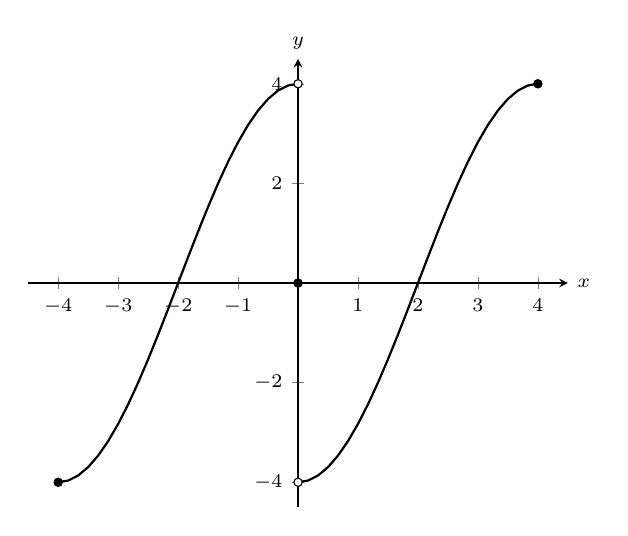
\begin{tikzpicture}
\begin{axis}[tick label style={font=\scriptsize},axis y line=middle,axis x line=middle,name=myplot,%
			xtick={-4,...,-1,1,2,...,4},% 
%			ytick={-6,-4,-2,0,2,4,6},
%			minor y tick num=1,
%			extra y ticks={-5,-3,...,7},%
			ymin=-4.5,ymax=4.5,%
			xmin=-4.5,xmax=4.5%
]

%\addplot [thick,{\colorone},smooth,domain=0:.9] {1/(x-1)^2};
%\addplot [{\colorone},thick,smooth,domain=1.1:2] {1/(x-1)^2};
\addplot [thick,{\colorone},domain=-4:0] {4*cos(deg(x)*3.14159/4};
\addplot [thick,{\colorone},domain=0:4]  {-4*cos(deg(x)*3.14159/4};
%
\fill[black,draw=black] (axis cs:0,0) circle (1.5pt);
\fill[white,draw=black] (axis cs:0,4) circle (1.5pt);
\fill[black,draw=black] (axis cs:-4,-4) circle (1.5pt);
\fill[black,draw=black] (axis cs:4,4) circle (1.5pt);
\fill[white,draw=black] (axis cs:0,-4) circle (1.5pt);
\end{axis}
\node [right] at (myplot.right of origin) {\scriptsize $x$};
\node [above] at (myplot.above origin) {\scriptsize $y$};
\end{tikzpicture}
\end{minipage}

\noindent\begin{minipage}[t]{.5\linewidth}
\begin{enumerate}
\item		$\ds \lim_{x\to 0^-} f(x)$
\item		$\ds \lim_{x\to 0^+} f(x)$
\end{enumerate}
\end{minipage}
\noindent\begin{minipage}[t]{.5\linewidth}
\begin{enumerate}\addtocounter{enumii}{2}
\item		$\ds \lim_{x\to 0} f(x)$
\item		$f(0)$
%\item		$\ds \lim_{x\to 2^-} f(x)$
%\item		$\ds \lim_{x\to 0^+} f(x)$
\end{enumerate}
\end{minipage}
}

\item {
\noindent\begin{minipage}{\linewidth}\centering
\begin{tikzpicture}
\begin{axis}[tick label style={font=\scriptsize},axis y line=middle,axis x line=middle,name=myplot,%
			xtick={-4,...,-1,1,2,...,4},% 
%			ytick={-6,-4,-2,0,2,4,6},
%			minor y tick num=1,
%			extra y ticks={-5,-3,...,7},%
			ymin=-4.5,ymax=4.5,%
			xmin=-4.5,xmax=4.5%
]

%\addplot [thick,{\colorone},smooth,domain=0:.9] {1/(x-1)^2};
%\addplot [{\colorone},thick,smooth,domain=1.1:2] {1/(x-1)^2};
\addplot [thick,{\colorone}] coordinates {(-4,0) (-2,2) (0,0) (2,2) (4,0)}; 
%\addplot [thick,{\colorone},domain=0:4]  {-4*cos(deg(x)*3.14159/4};
%
\fill[black,draw=black] (axis cs:0,0) circle (1.5pt);
\fill[black,draw=black] (axis cs:-4,0) circle (1.5pt);
\fill[black,draw=black] (axis cs:-2,0) circle (1.5pt);
\fill[white,draw=black] (axis cs:-2,2) circle (1.5pt);
\fill[white,draw=black] (axis cs:2,2) circle (1.5pt);
\fill[black,draw=black] (axis cs:4,0) circle (1.5pt);
\end{axis}
\node [right] at (myplot.right of origin) {\scriptsize $x$};
\node [above] at (myplot.above origin) {\scriptsize $y$};
\end{tikzpicture}
\end{minipage}

\noindent\begin{minipage}[t]{.5\linewidth}
\begin{enumerate}
\item		$\ds \lim_{x\to -2^-} f(x)$
\item		$\ds \lim_{x\to -2^+} f(x)$
\item		$\ds \lim_{x\to -2} f(x)$
\item		$f(-2)$
\end{enumerate}
\end{minipage}
\noindent\begin{minipage}[t]{.5\linewidth}
\begin{enumerate}\addtocounter{enumii}{4}
\item		$\ds \lim_{x\to 2^-} f(x)$
\item		$\ds \lim_{x\to 2^+} f(x)$
\item		$\ds \lim_{x\to 2} f(x)$
\item		$f(2)$
\end{enumerate}
\end{minipage}
}


\item {
\noindent\begin{minipage}{\linewidth}\centering
\begin{tikzpicture}
\begin{axis}[tick label style={font=\scriptsize},axis y line=middle,axis x line=middle,name=myplot,%
			xtick={-4,...,-1,1,2,...,4},% 
%			ytick={-6,-4,-2,0,2,4,6},
%			minor y tick num=1,
%			extra y ticks={-5,-3,...,7},%
			ymin=-4.5,ymax=4.5,%
			xmin=-4.5,xmax=4.5%
]
\draw [thick,{\colorone}] (axis cs:-4,-4) -- (axis cs:-3,-4);
\draw [thick,{\colorone}] (axis cs:-3,-3) -- (axis cs:-2,-3);
\draw [thick,{\colorone}] (axis cs:-2,-2) -- (axis cs:-1,-2);
\draw [thick,{\colorone}] (axis cs:-1,-1) -- (axis cs:0,-1);
\draw [thick,{\colorone}] (axis cs:0,0) -- (axis cs:1,0);
\draw [thick,{\colorone}] (axis cs:1,1) -- (axis cs:2,1);
\draw [thick,{\colorone}] (axis cs:2,2) -- (axis cs:3,2);
\draw [thick,{\colorone}] (axis cs:3,3) -- (axis cs:4,3);

%
\fill[black,draw=black] (axis cs:-4,-4) circle (1.5pt);
\fill[white,draw=black] (axis cs:-3,-4) circle (1.5pt);
\fill[black,draw=black] (axis cs:-3,-3) circle (1.5pt);
\fill[white,draw=black] (axis cs:-2,-3) circle (1.5pt);
\fill[black,draw=black] (axis cs:-2,-2) circle (1.5pt);
\fill[white,draw=black] (axis cs:-1,-2) circle (1.5pt);
\fill[black,draw=black] (axis cs:-1,-1) circle (1.5pt);
\fill[white,draw=black] (axis cs:0,-1) circle (1.5pt);
\fill[black,draw=black] (axis cs:0,0) circle (1.5pt);
\fill[white,draw=black] (axis cs:1,0) circle (1.5pt);
\fill[black,draw=black] (axis cs:1,1) circle (1.5pt);
\fill[white,draw=black] (axis cs:2,1) circle (1.5pt);
\fill[black,draw=black] (axis cs:2,2) circle (1.5pt);
\fill[white,draw=black] (axis cs:3,2) circle (1.5pt);
\fill[black,draw=black] (axis cs:3,3) circle (1.5pt);
\fill[white,draw=black] (axis cs:4,3) circle (1.5pt);
\end{axis}
\node [right] at (myplot.right of origin) {\scriptsize $x$};
\node [above] at (myplot.above origin) {\scriptsize $y$};
\end{tikzpicture}
\end{minipage}

Let $-3\leq a\leq 3$ be an integer.

\noindent\begin{minipage}[t]{.5\linewidth}
\begin{enumerate}
\item		$\ds \lim_{x\to a^-} f(x)$
\item		$\ds \lim_{x\to a^+} f(x)$
\end{enumerate}
\end{minipage}
\noindent\begin{minipage}[t]{.5\linewidth}
\begin{enumerate}\addtocounter{enumii}{2}
\item		$\ds \lim_{x\to a} f(x)$
\item		$f(a)$\end{enumerate}
\end{minipage}
}

\end{enumerate}

\begin{sol}
\begin{enumerate}
\item {\begin{enumerate}
\item		2
\item		2
\item		2
\item		1
\item	 	As $f$ is not defined for $x<0$, this limit is not defined.
\item		1
\end{enumerate}}
\item {\begin{enumerate}
\item		1
\item		2
\item		Does not exist.
\item		2
\item		0
\item	 	As $f$ is not defined for $x<0$, this limit is not defined.
\end{enumerate}
}
\item {\begin{enumerate}
\item		Does not exist.
\item		Does not exist.
\item		Does not exist.
\item		Not defined.
\item		0
\item	 	0
\end{enumerate}
} 
\item {\begin{enumerate}
\item		2
\item		0
\item		Does not exist.
\item		1
\end{enumerate}
}
\item {\begin{enumerate}
\item		2
\item		2
\item		2
\item		2
\end{enumerate}
}
\item {\begin{enumerate}
\item		4
\item		$-4$
\item		Does not exist.
\item		0
\end{enumerate}
}
\item {\begin{enumerate}
\item		2
\item		2
\item		2
\item		0
\item		2
\item		2
\item		2
\item		Not defined

\end{enumerate}
}
\item  {\begin{enumerate}
\item		$a-1$
\item		$a$
\item		Does not exist.
\item		$a$
\end{enumerate}
}
\end{enumerate}
\end{sol}

\end{ex}
% % % % % % % % % % % %
% % % % % % % % % % %
\begin{ex}
\begin{enumerate}
\item 
\item 
\item 
\item 
\end{enumerate}

\begin{sol}
\begin{enumerate}
\item 
\item 
\item 
\item 
\end{enumerate}
\end{sol}

\end{ex}
% % % % % % % % % % % %



%%%%%%%%%%
\begin{ex}
Use a calculator to estimate $\ds\lim_{x\to 0}
\frac{\sin x}{x}$, where $x$ is in radians.
\end{ex}

%%%%%%%%%%
\begin{ex}
Use a calculator to estimate $\ds\lim_{x\to 0}
\frac{\tan(3x)}{\tan(5x)}$, where $x$ is in radians.
\end{ex}

%%%%%%%%%%
\begin{ex}
Use a calculator to estimate $\ds\lim_{x\to 1^{+}}\frac{|x-1|}{1-x^2}$ and $\ds\lim_{x\to 1^{-}}\frac{|x-1|}{1-x^2}$.
\end{ex}

\end{enumialphparenastyle}

\end{multicols}